\documentclass[10pt]{article}
\usepackage[margin=0.5in]{geometry}
\usepackage{graphicx}
\usepackage{caption}
\usepackage{subcaption}
%Gummi|065|=)
\title{\textbf{CS267 HW1-Matrix Multiple}}
\author{Joao (SID: ) \& Haoyu Chen (SID: 23269048)}
\date{}
\begin{document}

\maketitle

\section{Introduction}
\section{The Best Implement}
In this section, we first describ the implement details of our best edition. Then we illustrate some benchemark results.
\subsection{The Implement details}
Our best implement edition is using SSE vectorization, loop unroll, matrix block and padding. The Fig.~1 illustrates the roadmap of our implement. We use L1 cache blocking to decrease the miss hit rate. We find the optimal block size for one matrix is 64 * 64 doubles (i.e. 32KB). For each submatrix, we use SSE and loop unroll to do the matrix multiple, see Fig~.1. \\
\\
If data is aligned in the memory or cache, it will make the vector computing faster, because the each load data from memory can include useful information as much as possible. Thus, we allocate some temporary memory to hold the submatrices data, which is saved aligned. Another reason that we copy data to the temporary is that we can do padding easily, which simplify the code and increase the cache hit rate. The details of memory copy can be found in Fig.~2. Since there are three loops for the each submatrix, if we copy data in the innermost loop, that would be very redundant. Thus, we copy one big chunk of matrix B in the first loop, copy chunk of A in the second loop, and chunk C in the third loop. When we copy the data, we pad the matrice so that their dimensions are the integer times of 4.\\   
\begin{figure}[h!]
  \centering
      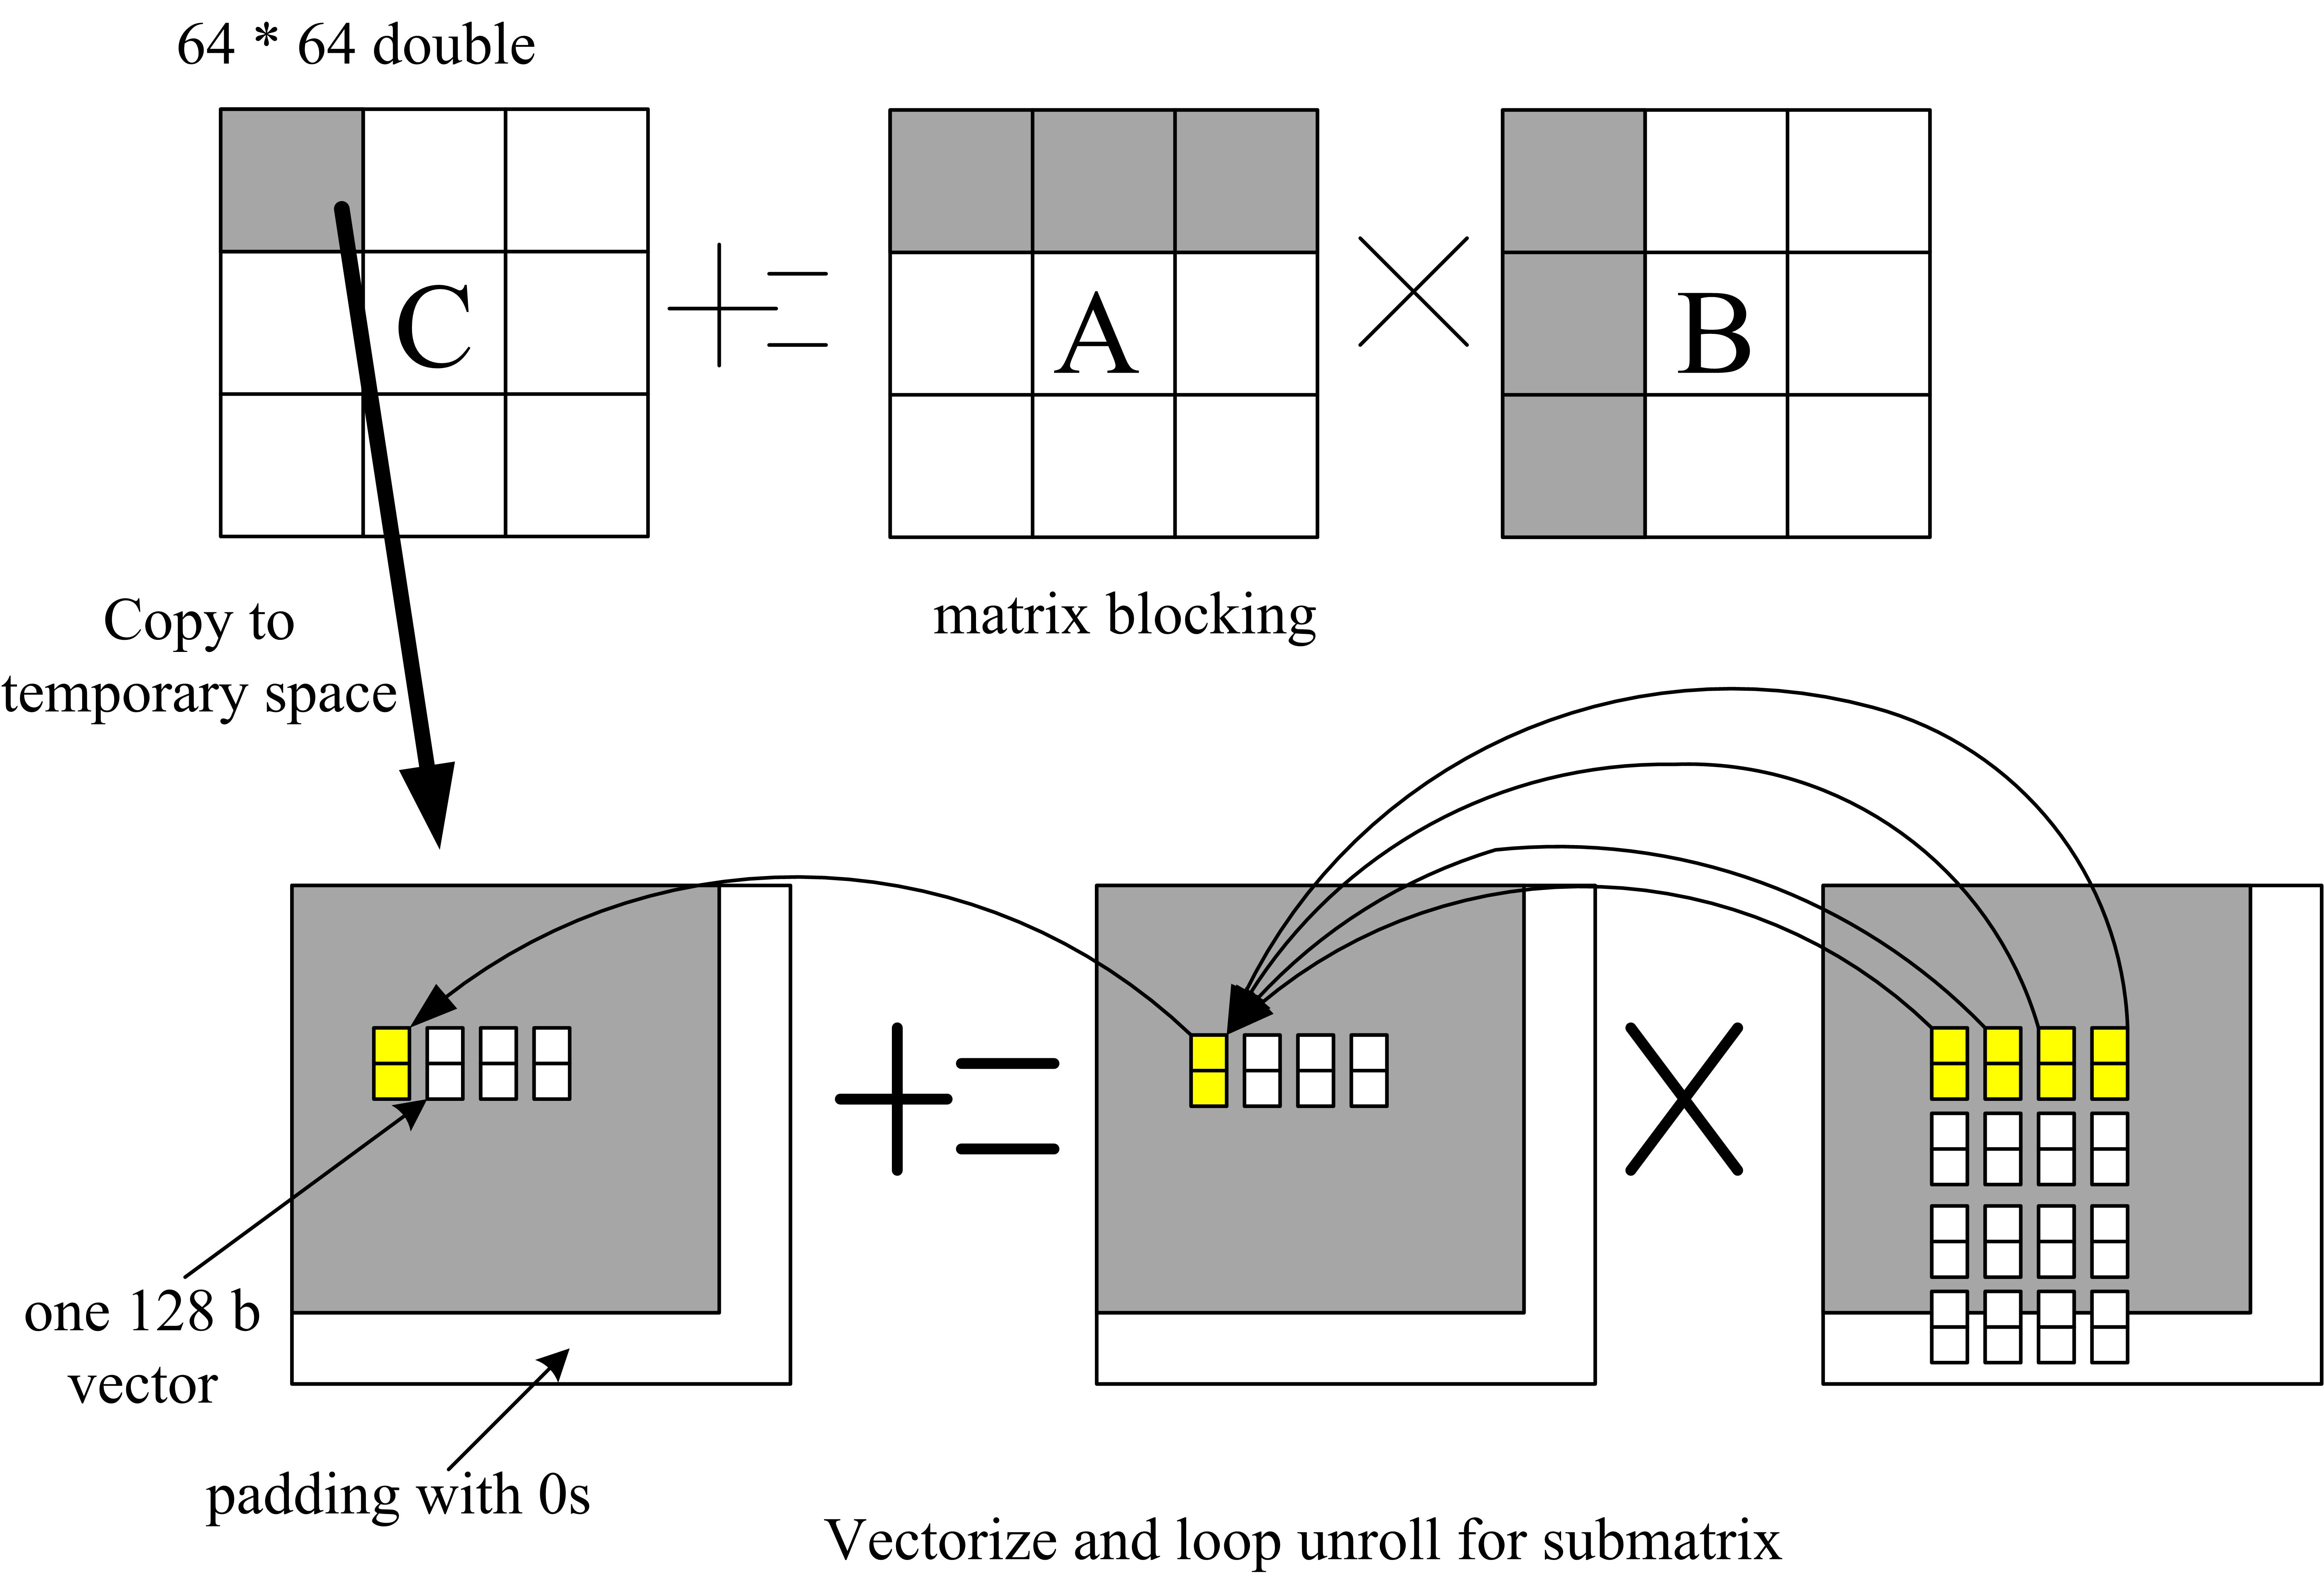
\includegraphics[width=0.6\textwidth]{267_1_1.jpg}
  \caption{roadmap of the best implement}
\end{figure}
\\
After we copy the data into the temporary memory, we multiple the submatrice with SSE vectorization. Since the size of register is 128 bit, each vector can load 2 doubles. Meanwhile, we also apply the loop unroll in this stage. We load 4 vectors for submatrix C and A, and 16 vectors for matrix B. And we do calculation of these vector in one iteration. The loop unroll brings big improvement for our program. There are two reasons for this significant improvement: 1) the loop unroll decrease the redundent computing and can make the CPU run it with automatically parallel; 2) the loop unroll here can also be viewed as one more level blocking (register blocking). After we finish the computing of submatrix multiple, the results are copied back to the original address.\\  
\begin{figure}[h!]
  \centering
      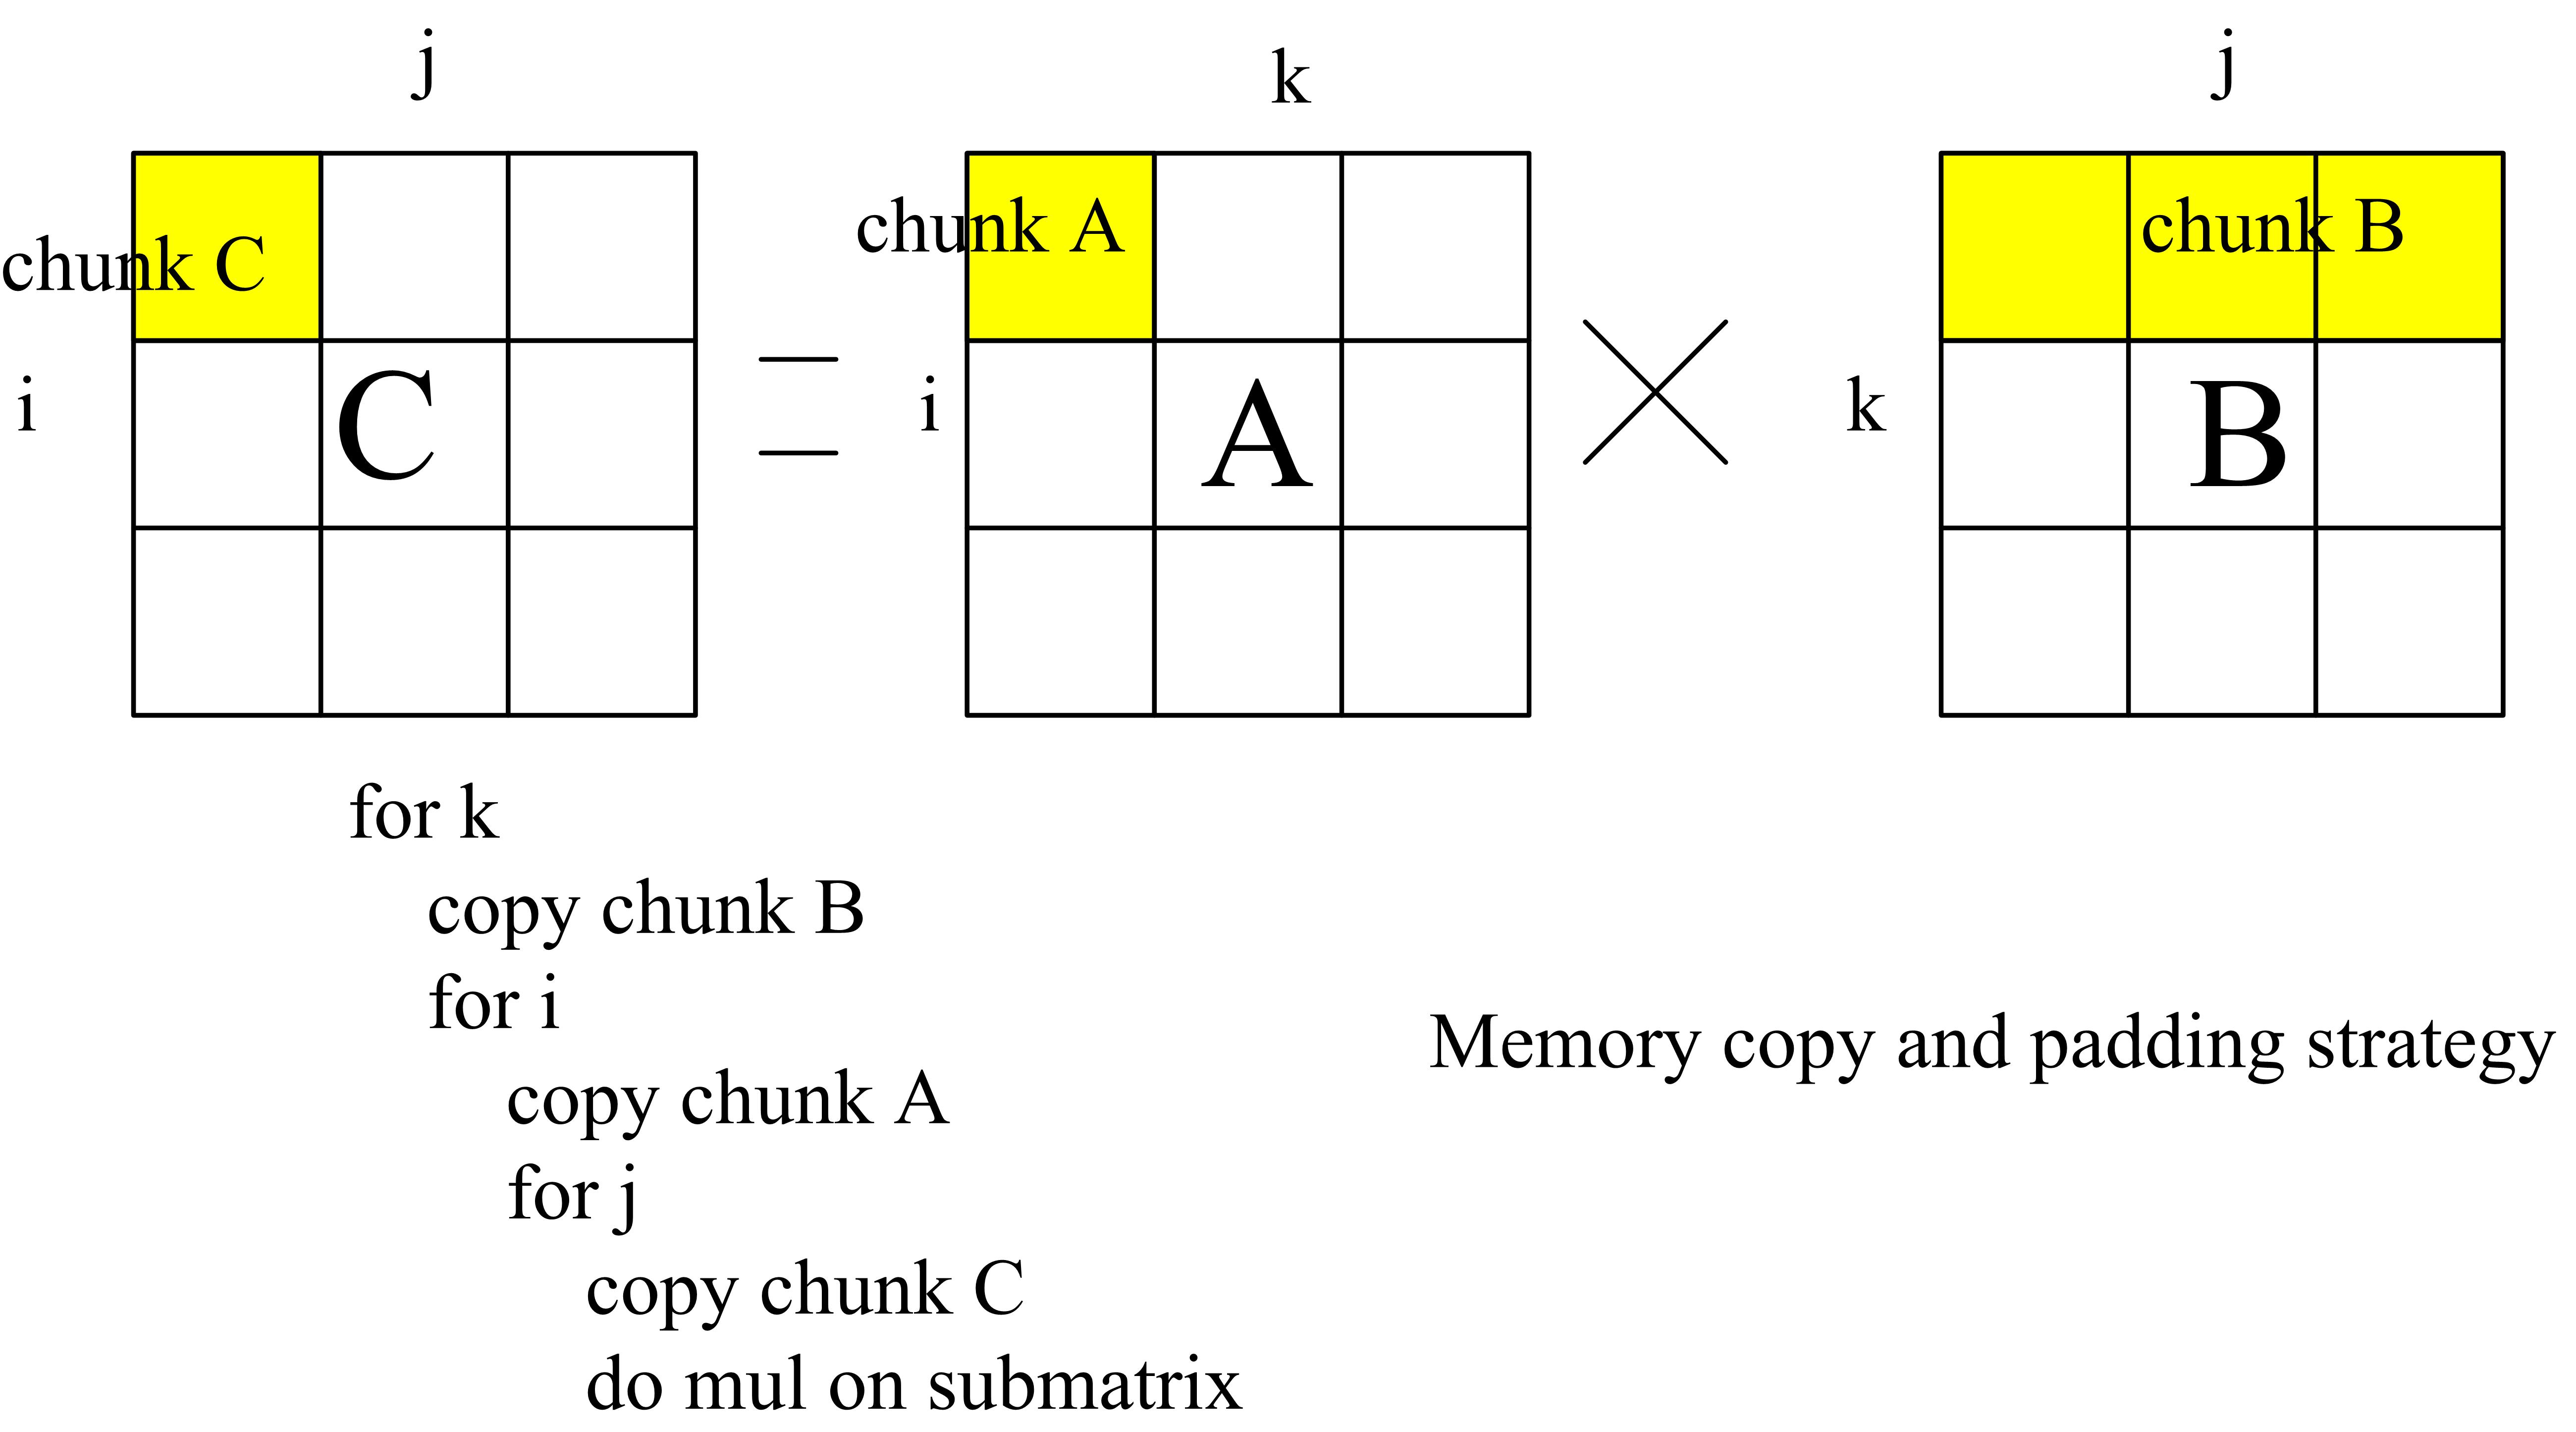
\includegraphics[width=0.6\textwidth]{267_1_2.jpg}
  \caption{memory copy}
\end{figure}
\subsection{Benchmark}
In this part, we compare the performace for our different implements. Fig.~3 shows the peak performance percentage of different implements for matrix size varying from 31 to 769. We can find that just try SSE can just increase the performace a little. But with adding blocking, the performance improved significant. Another significant is the loop unroll, espencially we unroll it by 4. Just as we disussed above, the unroll can act like register blocking, which we think it's the main reason that it increases the percentage so much. Finally, out best implement achieves 53\%.
\begin{figure}[h!]
  \centering
      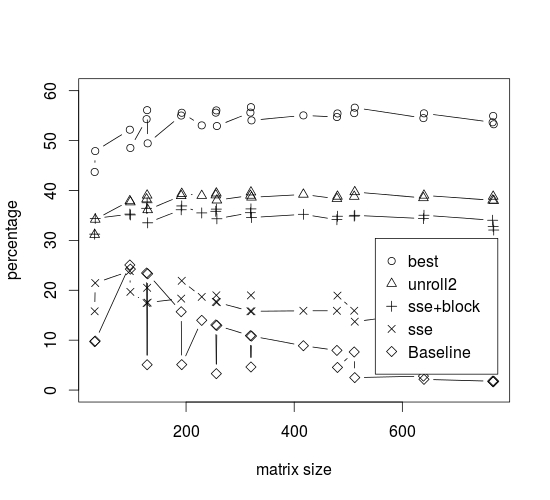
\includegraphics[width=0.6\textwidth]{result.jpeg}
  \caption{benchmark of performance}
\end{figure}

\section{Other Solutions}
\subsection{Matrix Transpose}
\subsection{Recursive Multiple and Strassen}
We also tried multiple matrice recursively and Strassen algorithm. Their performance can be seen Fig.~4. The performance of recursive method is really bad. We think it's so bad, because the program keep construct the stack and delete stack which decrease the efficieny significantly. And another reason is that the performace of recursive method depends on the threhold to stop the recursive and use normal matrix multiple, which is hard to tune. \\
\\
The efficiency of Strassen method is also very low, because 1) in order to implement this method, I copy the submatrice to the temporary memory, which increase the memory traffic; and 2) there are a big constant cost before we achieve the Big-O performance.   

\begin{figure}[h!]
  \centering
      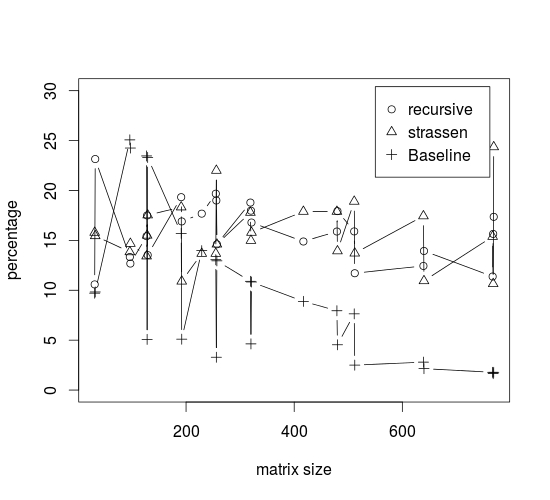
\includegraphics[width=0.6\textwidth]{result_2.jpeg}
  \caption{benchmark of performance}
\end{figure}
\section{Conclusion}


\end{document}
